I% Chapter Template

\chapter{Vector Structure and Operations} % Main chapter title

\label{VectorStructure} % Change X to a consecutive number; for referencing this chapter elsewhere, use \ref{ChapterX}

\lhead{Vector Structure. \emph{Vector Structure}} % Change X to a consecutive number; this is for the header on each page - perhaps a shortened title

%----------------------------------------------------------------------------------------
%	SECTION - Radix Balanced Vectors
%----------------------------------------------------------------------------------------

\section{Radix Balanced Vectors}

%-----------------------------------
%	SUBSECTION - Tree structure
%-----------------------------------

\subsection{Tree structure}
% describe tree: balancing, filling, block sizes
% why structure helps with operations implementation 
% hint why radix?  


\begin{figure}[h!]
  \centering
  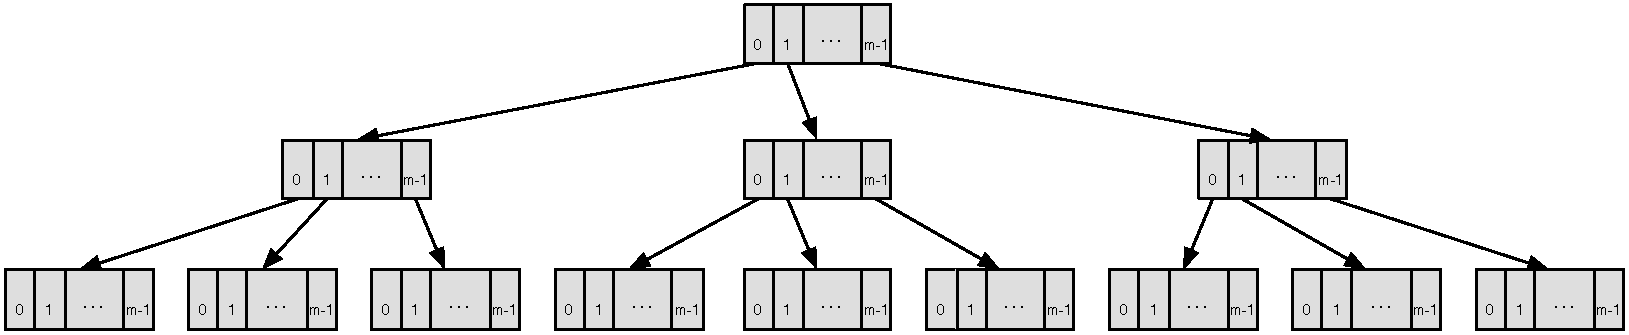
\includegraphics[width=\textwidth]{Figures/Radix_Balanced}
  \label{badix_balanced}
  \caption{Radix Balanced Tree Structure}
\end{figure}



%-----------------------------------
%	SUBSECTION - Operations
%-----------------------------------
\subsection{Operations}
% List core operations
The immutable \texttt{Vector} \cite{scalaVector211} is a subtype of \texttt{IndexedSeq} in the current Scala collections, as such it implements all operations defined on it. Most operations are implemented using a set of core operations that can be implemented efficiently on RB-Trees, those operations are: \texttt{apply}, \texttt{updated}, \texttt{append}, \texttt{prepend}, \texttt{drop} and \texttt{take}. 

% performance log_{32}(n) -> effective constant time
The performances of most operations on RB-Trees have a computational complexity of $O(log_{32}(n))$, equivalent to the height of the tree. This is usually referred as effective constant time because for 32 bit signed indices the height of the tree will bounded by a small constant (6.2 in the case of books of size 32). This bound is reasonable to ensure that in practice the operations behave like constant time operations.  
 
% naive implementation just as high level guide
% hint of displays and transient states
In this section the operations will be presented on a high level\footnote{Ignoring some pieces of code like casts, return types, type covariance, among others.} and without optimisation. These reflect the worst case scenario or the base implementation that is used before adding optimizations (see chapter \ref{Optimizations}). To improve performance of some operations, displays are used on branches of the RB-Tree (see section \ref{sec:Displays}). To improve the complexity of operations to amortized constant time (instead of effective constant time\footnote{In this context, effective constant time has a large but bounded constant time complexity, while amortized constant time tends to have a bound closer to a one level tree update.}) for some operation sequences the vectors are augmented with transient states.

%-----------------------------------
%	SUBSUBSECTION - Apply
%-----------------------------------

\subsubsection{Apply}
% used in head and last
The \texttt{apply} operation in indexed sequences is defined as the operation that gets the element located at some index. This is the main element access method and it is used in other methods such as \texttt{head} and \texttt{last}.

\begin{lstlisting}[frame=single]
def apply(index: Int): A = {
  def getElem(node: Array[AnyRef], depth: Int): A = {
    val indexInNode = // compute index
    if(depth == 1) node(indexInNode)
    else getElem(node(indexInNode), depth-1) 
  }
  getElem(vectorRoot, vectorDepth)
}
\end{lstlisting}

% performance log_{32}(n), hint of displays
The base implementation on RB-Trees of this operation requires a simple traversal from the root to the leaf containing the element. Where the path taken is defined by the index of the element and extracted using some efficient bitwise operations (see section \ref{ComputingIndices}). With this traversal of the tree, the complexity of the \texttt{apply} operation is $O(log_{32}(n))$. This complexity can be reduced for some subset of elements by adding displays.


%-----------------------------------
%	SUBSUBSECTION - Updated
%-----------------------------------

\subsubsection{Updated}
% base implementation needs to update the whole branch
The \texttt{updated} method returns a new immutable \texttt{Vector} with one updated element at a given index. This is the core operation to modify the contents of the vector. 

On immutable RB-Trees the updated operation has to recreate the whole branch from the root to the element being updated. The update of the leaf creates a fresh copy of the leaf with the updated element. Then the parent of the leaf also need to create a new node with the updated reference to the new leaf, and so on up to the root. 

\begin{lstlisting}[frame=single]
def updated(index: Int, elem: A) = {
  def updatedNode(node: Array[AnyRef], depth: Int) = {
    val indexInNode = // compute index
    val copy = clone(node)
    if(depth == 1) {
      copy(indexInNode) = elem
    } else {
      copy(indexInNode) = 
        updatedNode(node(indexInNode), depth-1)
    }
    copy
  }
  new Vector(updatedNode(vectorRoot, vectorDepth), ...)
}
\end{lstlisting}

% with transient states, local updates can be amortised
Therefore the complexity of this operation is $O(log_{32}(n))$, for the traversal and creation of each node in the brach. This operation can be improved to have amortized constant time updates for local updates using displays with transient states. This way the parent nodes are only updated lazily when absolutely necessary. For example, if some leaf has all it's elements updated from left to right, the leaf will be copied as many times as there are updates, but the parent of that leaf does not change during those operations.

%-----------------------------------
%	SUBSUBSECTION - Additions
%-----------------------------------

\subsubsection{Extentions}
The main operations to extend an immutable \texttt{Vector} are \texttt{append} and \texttt{prepend} a single element. Those operations are considered the main ones because they have efficient implementations on RB-Trees. Other operations like \texttt{concatenated} and \texttt{insert} are also present, but usually avoided because of performance.


\paragraph{Append}
% base implementation needs to update the whole branch
To append an element on the tree there are two main cases, the last leaf of the tree is not full or it is full. If the last leaf is not full the element is inserted at the end of it and all nodes of the last branch are updated. Or, if the leaf is full we must find the lowest node in the last branch where there is sill room left for a new branch. Then a new branch is appended to it, down to the a new leaf with the element being appended. 

In both cases the new \texttt{Vector} object will have the end index increased by one. When the root is full, the depth of the vector will also increase by one.

\begin{lstlisting}[frame=single]
def :+(elem: A): Vector[A] = {
  def append(node: Array[AnyRef], depth: Int) = {
    if (depth == 1) 
      cloneAndAppend(node, elem)
    else if (!isTreeFull(node.last, depth-1)) 
      cloneAndUpdateLast(node, append(node.last, depth-1))
    else
      cloneAndAppend(node, newBranch(depth-1))
  }
  def createNewBranch(depth: Int): Array[AnyRef] = {
    if (depth == 1) Array(elem)
    else Array(newBranch(depth-1))
  }
  if(!isTreeFull(root, depth))) 
    new Vector(append(root, depth), depth, ...)
  else 
    new Vector(Array(root, newBranch(depth)), depth+1, ...)
}
\end{lstlisting}

Where the \texttt{isTreeFull} operation computes the answer using efficient bitwise operations on the end index of the vector.

% performance log_32(n), hint of transient to amortise consecutive appends are amortised
Due to the update of all nodes in the last branch, the complexity of this operation is $O(log_{32}(n))$. This complexity can be amortized to constant time using displays with transient states for consecutive append operations on the vector (see section \ref{sec:DisplaysTransient}).

\paragraph{Prepend}
% base implementation needs to update the whole branch
The key to be able to prepend  elements to the tree is the additional \texttt{startIndex} that the vector keeps. Without this it would be impossible to prepend an element to the vector without a full copy of the vector to rebalance the RB-Tree. The operation can be split into to cases depending on the value of the start index.

% shift top and start index
The first case is to prepend an element on a vector that start at index 0. If the root is full, create a new root on top with the old root as branch at index 1. If there is still space in the root, shift branches in the root by one to the right. In both sub\-cases, create a new branch containing nodes of size 32, but with only the last branch assigned. Put the element in the last position of this newly created branch and set the start index of the vector to that index in the tree.

The second case is to prepend an element on a vector that has a non zero start index. Follow the branch of the start index minus one from the root of the tree. If it reaches the a leaf, prepend the element to that leaf. If it encounters an inexistent branch, create it by putting the element in its rightmost position and leaving the rest empty. In both sub\-cases update the parent nodes up to the root.

The new \texttt{Vector} object will have an updated start index and end index. to account for the changes in the structure of the tree. It may also have to increase the depth of the vector if the start index was previously zero. 

\begin{lstlisting}[frame=single]
def +:(elem: A): Vector[A] = {
  def prepended(node: Array[AnyRef], depth: Int) = {
    val indexInNode = // compute index
    if (depth == 1) 
      cloneAndUpdate(node, indexInNode, elem)
    else 
      cloneAndUpdate(node, indexInNode, 
                prepended(node(indexInNode), depth-1))
  }
  def newBranch(depth: Int): Array[AnyRef] = {
    val newNode = new Array[AnyRef](32)
    newNode(31) = 
      if (depth == 1) elem 
      else newBranch(depth-1)
    newNode
  }
  if(startIndex==0) {
    new Vector(Array(newBranch(depth), root), depth+1, ...)
  } else {
    new Vector(prepended(root, depth), depth, ...)  
  }
}
\end{lstlisting}

% performance log_32(n), hint of transient to amortise consecutive prepends are amortised
Due to the update of all nodes in the first branch, the complexity of this operation is $O(log_{32}(n))$. This complexity can be amortized to constant time using displays with transient states for consecutive append operations on the vector (see section \ref{sec:DisplaysTransient}).


\paragraph{Concatenation and Insert}
% describe high level implementation in vector
%% describe branch rebalancing 
% performance O(n)
Given that elements in an RB-Tree are densely packed, the it is only possible to implement efficient element append and prepend.


%-----------------------------------
%	SUBSUBSECTION - Splits
%-----------------------------------

\subsubsection{Splits}
% used in tail, init, take, takeRight, drop, dropRight
% describe implementation in vector
% performance log_32(n) 


%----------------------------------------------------------------------------------------
%	SECTION - Parallel Vectors
%----------------------------------------------------------------------------------------

\section{Parallel Vectors}
% why are  parallel vector useful
% how are they paralellized (wraps an vector)
% why do they suffer performance wise (no efficient concat)
% fork-join pool

%-----------------------------------
%	SUBSUBSECTION - Splitter
%-----------------------------------

\subsection{Splitter (Iterator)}
% split into half 
To divide the work into tasks for thread pool, a splitter is used to iterate over all elements of the collection. Splitters are a special kind of iterator that can be split at any time into some partition of the remaining elements. In the case of sequences the splitter should retain the original order. The most common implementation consists in dividing the remaining elements into two half. 

The current implementation of the immutable parallel  vector \cite{scalaParVector211}  uses the common division into 2 parts for it splitter. The drop and take operations are used divide the vector for the two new splitters.

%-----------------------------------
%	SUBSUBSECTION - Combiner
%-----------------------------------

\subsection{Combiner (Builder)}
% lazy combiner
Combiners are used to merge the results from different tasks (in methods like map, filter, collect, ...) into the new collection. Combiners are a special kind of builder that is able to merge to partial results efficiently. When it's impossible to implement efficient combination operation, usually a lazy combiner is used. The lazy combiner is one keeps all the it's sub-combiners in an array buffer and only when the end result is needed they are combined. This is a fairly efficient implementation but does not take full advantage of parallelism. 

The current implementation of the immutable parallel vector \cite{scalaParVector211} use the lazy approach because of it's inefficient concatenation operation. One of the consequences of this is that the parallel operations will always be bounded by this sequential combination of elements, which can be beaten by the sequential version in many cases.
 

%----------------------------------------------------------------------------------------
%	SECTION - Relaxed Radix Balanced Vectors
%----------------------------------------------------------------------------------------

\section{Relaxed Radix Balanced Vectors}

%-----------------------------------
%	SUBSECTION - Tree structure
%-----------------------------------

\subsection{Relaxed Tree structure}
% describe tree: balancing, filling, block sizes
% describe sizes array and where it is kept (change from left to right for indexing simplification)
% mention size of nodes and null sizes
% unbalanced trees can only be generated by concatenation, and splits

\begin{figure}[h!]
  \centering
  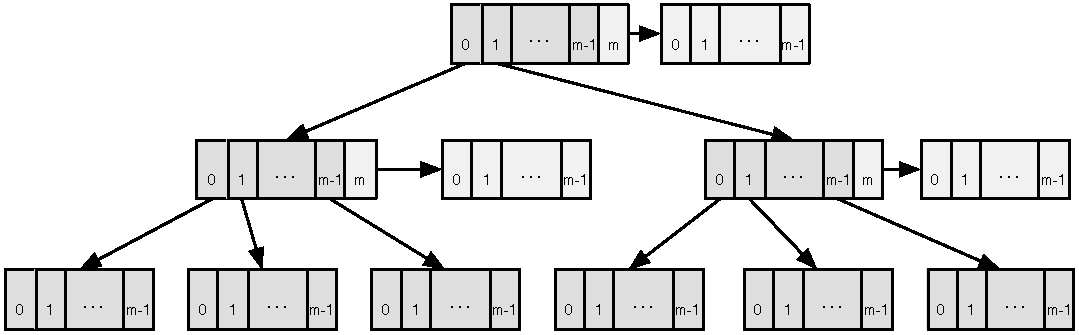
\includegraphics[width=\textwidth]{Figures/Relaxed_Radix_balanced}
  \label{Relaxed_Radix_balanced}
  \caption{Radix Balanced Tree}
\end{figure}

\begin{figure}[h!]
  \centering
  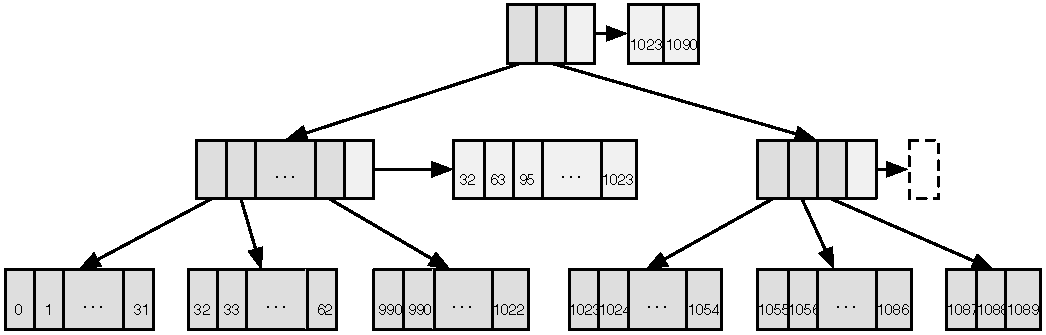
\includegraphics[width=\textwidth]{Figures/Relaxed_radix_example}
  \label{Relaxed_radix_example}
  \caption{Relaxed radix example}
\end{figure}

%-----------------------------------
%	SUBSECTION - Operations
%-----------------------------------
\subsection{Relaxed Operations}
% describe how the implementation uses relaxed radix when necessary and uses radix based operation when possible

%-----------------------------------
%	SUBSUBSECTION - Apply
%-----------------------------------

\subsubsection{Apply (get element at index)}
% describe the way to get the node indices in an unbalanced node


%-----------------------------------
%	SUBSUBSECTION - Updated
%-----------------------------------

\subsubsection{Updated}
% doesn't change much, the sizes do not need to be updated, they jus need to be copied. Going to the correct position still may needs to access the sizes.

%-----------------------------------
%	SUBSUBSECTION - Additions
%-----------------------------------

\subsubsection{Joins}

%-----------------------------------
\paragraph{Append}
% difference is that the the sizes may need to be updated
% performance log_32(n), remind hint of transient to amortise consecutive appends are amortised

\paragraph{Prepend}
% describe different implementation
% hint the 


%-----------------------------------
\paragraph{Concatenation}
% describe high level implementation in rrbvector
%% describe branch rebalancing 
% performance log_32(n)

\begin{figure}[h!]
  \centering
  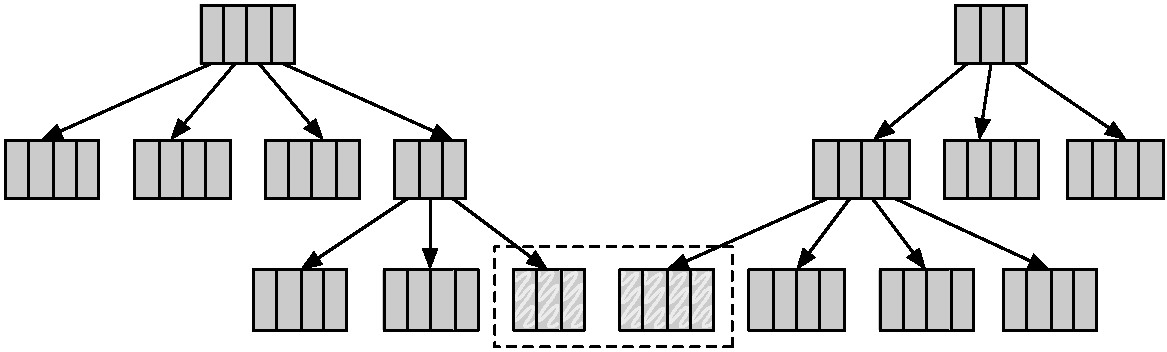
\includegraphics[width=\textwidth]{Figures/Concat0.pdf}
  \label{Concat0Benchmarks}
  \caption{Concatenation example with blocks of size 4: Rebalancing level 0}
\end{figure}

\begin{figure}[h!]
  \centering
  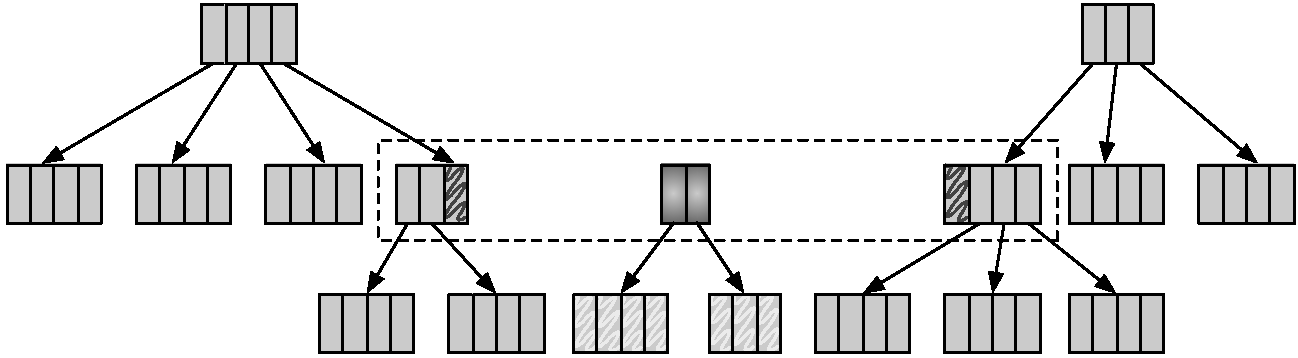
\includegraphics[width=\textwidth]{Figures/Concat1.pdf}
  \label{Concat1Benchmarks}
  \caption{Concatenation example with blocks of size 4: Rebalancing level 1}
\end{figure}

\begin{figure}[h!]
  \centering
  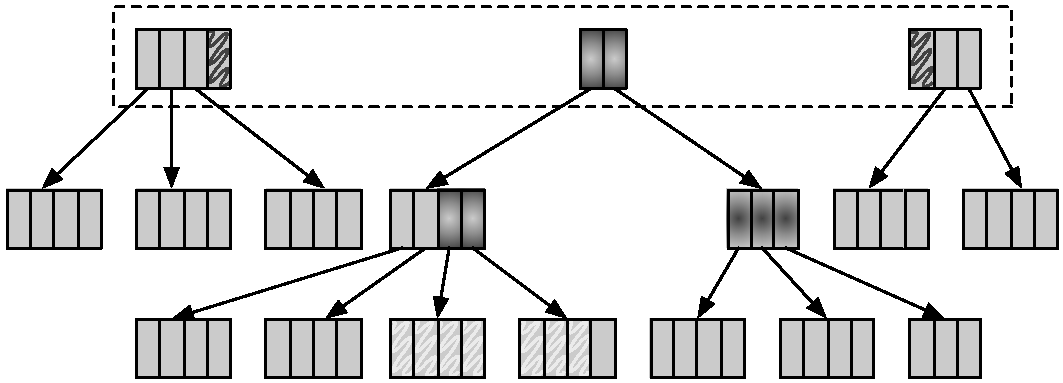
\includegraphics[width=\textwidth]{Figures/Concat2.pdf}
  \label{Concat2Benchmarks}
  \caption{Concatenation example with blocks of size 4: Rebalancing level 2}
\end{figure}

\begin{figure}[h!]
  \centering
  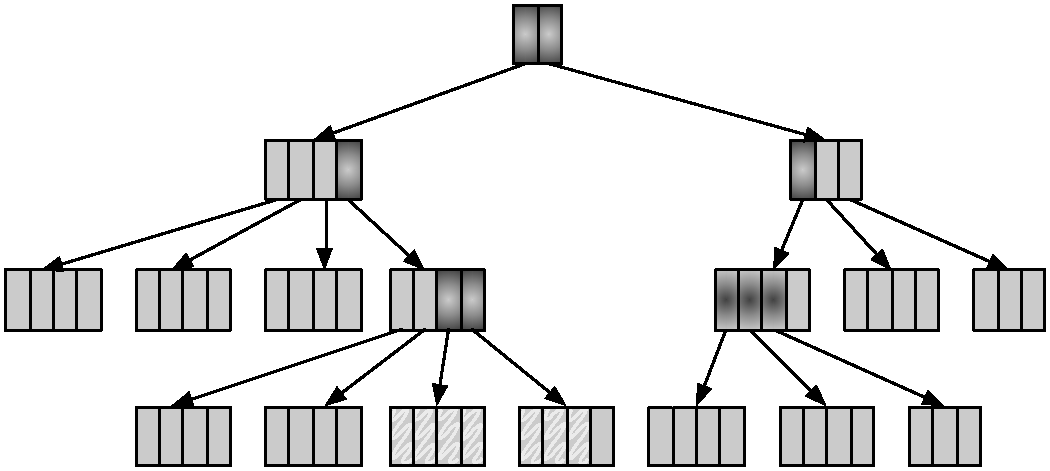
\includegraphics[width=\textwidth]{Figures/Concat3.pdf}
  \label{Concat3Benchmarks}
  \caption{Concatenation example with blocks of size 4: Rebalancing level 3}
\end{figure}


%-----------------------------------
\paragraph{Insert}
% new operation
% describe simple implementation using split and concat 
% performance log_32 (from split + concat)
% hint at possible optimization by inserting directly and using transient states (take advantage of locality)



%-----------------------------------
%	SUBSUBSECTION - Splits
%-----------------------------------

\subsubsection{Splits}
% used in tail, init, take, takeRight, drop, dropRight
% describe difference between the implementation (null and shift vs. cut and update size)

%-----------------------------------
%	SUBSUBSECTION - Splits
%-----------------------------------

\subsubsection{Parallel Vector}
% Combine: trivial expansion from builder
%% heuristic: try to construct balanced trees 
% Split into subtrees two, take the nearest power of 32 to the half


